% System Combination
% Harish K Krishnamurthy <www.ece.neu.edu/~hkashyap/>
\documentclass{article}

\usepackage[left=2cm, right=2cm, bottom=2cm, top=2cm]{geometry}
\usepackage{tikz}
\usetikzlibrary{shapes,arrows,shadows}
\usetikzlibrary{arrows.meta}
\tikzset{%
  >={Latex[width=2mm,length=2mm]},
  % Specifications for style of nodes:
            base/.style = {rectangle, rounded corners, draw=black,
                           minimum width=4cm, minimum height=1.3cm,
                            font=\sffamily},
  activityStarts/.style = {base, fill=blue!30},
       startstop/.style = {base, fill=red!30},
    result/.style = {base, fill=green!30},
         process/.style = {base, minimum width=2.5cm, fill=orange!15,
                           font=\ttfamily},
         myPoint/.style = {circle, fill=black, size=1pt},                  
}



\usepackage{amsmath,bm,times}
\newcommand{\mx}[1]{\mathbf{\bm{#1}}} % Matrix command
\newcommand{\vc}[1]{\mathbf{\bm{#1}}} % Vector command

\pagestyle{empty}  %% only pdf-picture, no page number
\begin{document}


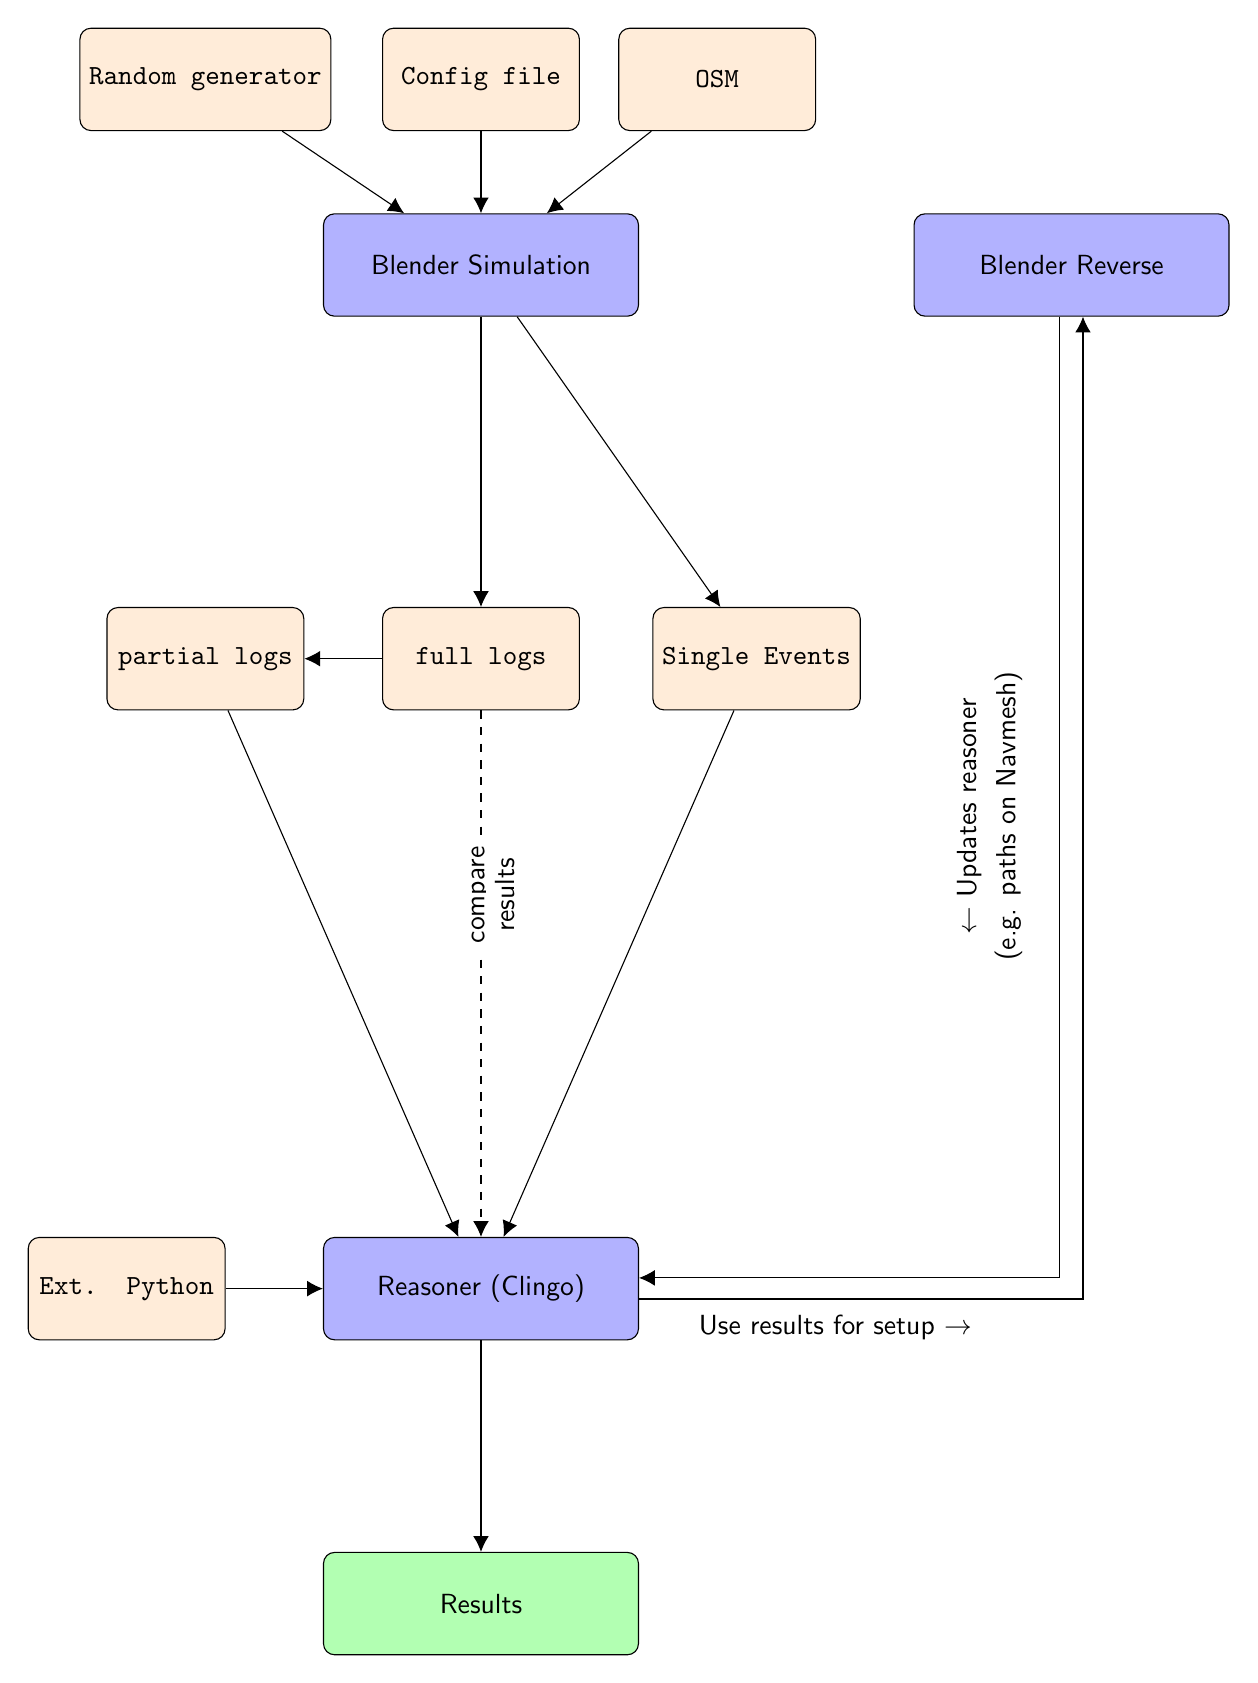
\begin{tikzpicture}[node distance=1.5cm,
    every node/.style={fill=white, font=\sffamily}]
  % Specification of nodes (position, etc.)

\node (blenderSim) at (6.5,0)            [activityStarts]              {Blender Simulation};
%\node (onCreateBlock)     [process, above of=blenderSim]          {onCreate()};

%\node (blenderReverse)    [activityStarts, right of=blenderSim, xshift=6cm]
%                                                              {Blender Reverse};
\node (blenderReverse) at (14, 0)   [activityStarts]  {Blender Reverse};                                                             
\path (blenderSim.north)+(-3.5,1.7) node (randGen) [process] {Random generator};
\path (blenderSim.north)+(0,1.7)  node (config)[process] {Config file};
\path (blenderSim.north)+(3,1.7)  node (osm)[process] {OSM};

\draw[->]     (randGen) -- (blenderSim);
\draw[->]     (config) -- (blenderSim);
\draw[->]     (osm) -- (blenderSim);

\node (singleEvents) at (10, -5) [process] {Single Events};
\node (fullogs) at (6.5, -5) [process] {full logs};
\node (partlogs) at (3, -5) [process] {partial logs};

\draw[->]     (blenderSim) -- (singleEvents);
\draw[->]     (blenderSim) -- (fullogs);
\draw[->]     (fullogs) -- (partlogs);

\node (reasoner) at (6.5,-13)    [activityStarts]     {Reasoner (Clingo)};
\node (external) at (2,-13)    [process]     {Ext. Python};

\draw[->]     (external) -- (reasoner);

\draw[->]             (singleEvents) -- (reasoner);
\draw[dashed,->]      (fullogs) -- (reasoner) ;
\node at (6.5, -8) [rotate=90] {compare};
\node at (6.8, -8) [rotate=90] {results};

\draw[->]      (partlogs) -- (reasoner);



\draw[->] ([xshift= -3cm] blenderReverse) |- ( [yshift=0.5cm] reasoner);
\draw[<-] ([xshift= 3cm] blenderReverse) |- ([yshift= -0.5cm] reasoner);
\node at (12.7, -7) [rotate=90] {$\leftarrow$ Updates reasoner};
\node at (13.2, -7) [rotate=90] {(e.g. paths on Navmesh)};

\node at (11, -13.5) { Use results for setup $\rightarrow$ };

\node (result) at (6.5,-17)    [result]     {Results};
\draw[->] (reasoner) -- (result);
\end{tikzpicture}



\end{document}
